\documentclass[11pt, english]{article}              
        \usepackage{geometry}
                \geometry{                          
                        a4paper,total={210mm,297mm},
                        tmargin=40.8mm,
                        bmargin=40.8mm,
                        lmargin=32.6mm,
                        rmargin=32.6mm,
                }

        \usepackage{titlesec}         
                \titleformat{\section}
                        {\normalfont\fontsize{18}{16}\bfseries}{\thesection}{0.5em}{}
                \titleformat{\subsection}
                        {\normalfont\fontsize{14}{16}\bfseries}{\thesubsection}{1em}{}
                \titleformat{\subsubsection}
                        {\normalfont\fontsize{11}{16}\bfseries}{\thesubsubsection}{1em}{}

        \usepackage{longtable}
        \usepackage{multirow}

        \usepackage[labelfont=bf,textfont=bf,font=small,skip=8pt]{caption}

        \setlength{\parindent}{0pt}
        \renewcommand{\baselinestretch}{1.25}
       	\usepackage{setspace}

        \usepackage{amsmath}
        \usepackage{amssymb}

	\usepackage{tikz}
                \usetikzlibrary{trees,arrows,topaths}
        
        \usepackage{graphicx}

\begin{document}

\pagenumbering{gobble}

        \title{\textsc{BF303 Management Developmet Program 3\\ Coursework Assignment}}
        \author{\textsc{Lewis Britton}}
        \date{\textsc{Academic Year 2019/2020}}
        \maketitle
        
        \begin{abstract}
		This report explores the issues present in the modern-day economy regarding low progression rate schools. Using a regression model we are able to view the variety of causal factors stemming from social and economic factors in relation to the background and environment of school pupils/students. The model moves through two sets of intermediary factors which account for the lost error value between the casual instruments and the overall effect. The primary intermediary factors take into account how the causes effect the overall situation in which pupils are found. The secondary intermediary factors extend these to personal social, economic and knowledge and understanding (K\&U) based attributes in the students’ home and educational life. These create an initially assumed strong model to judge progression issues. This model is used in the context of issues which are highlighted by various widening access teams around the UK who aim to increase progression rates from schools in the lowest ranked areas of deprivation. This is observed through the path of identifying and targeting needs and making an attempt to implement improvements through methods such as the Schools for Higher Education Programme (SHEP). This analysis explores different social and economic methods used under the idea of the SHEP and finds moderately successful data with many flaws with desperate room for social modelling improvement.
	\end{abstract}

\newpage

\pagenumbering{roman} 

	\renewcommand{\contentsname}{Table of Contents}

        \tableofcontents

\newpage

\pagenumbering{arabic}

\section{Background}

	It can be argued that there isn’t equal opportunity across schools, particularly within Glasgow/Scotland in this case. Many schools may be viewed from a linear perspective based on causal factors such as school reputation, historical results, affluence of students etc. However, there may be equal, if not greater, opportunity lurking in traditionally lower achieving schools. This may be disguised by many intermediary factors involving student mentality or even the teachers’ perspective or understanding regarding  their pupils; students who may not necessarily fit into their norm. The inclusion of these intermediary factors significantly affect a regressed model of future achievement (Koop, 2007).\\

	At the University of Strathclyde, the Widening Access team exists to aid this problem of mismatch on the path of causation. If we observe academic potential, or a semantically similar term, as the regressed variable, we see that observing only factors from standard or highly achieving schools leads to huge selection bias (Hindricks, Myles, 2013). Casual factors may include things such as the hierarchy of school reputation, school perception, general environment etc. (MacLeod, Urquiola, 2009). As described, these factors are plentiful in bias towards high progression rate, highly achieving schools. They fail to account for many differential factors. Factors which appear in an everlasting quantity, which perhaps may place students in lower achieving schools but do not directly affect their grades. Hence, their observed reputation is poor but at closer look, their real reputation is good and must be identified. Some factors held by underachieving schools include things like low family income, requirement to care, family surrounding, mental stability lack of belief and so on.\\

	The role of Strathclyde’s Widening Access Team is to highlight these intermediary factors within underachieving schools and utilise their tools and resources to optimise potential within these factors. Therefore, automatically selecting viable candidates from otherwise unexplored parts of the traditional causal portion of the academic potential regression. That is, identifying deserving students from low and poor progression rate schools in order to equalise them equivalents attending higher progression rate schools. Using tools such as the One Day Event we observe randomised control trials (MacLeod, Urquiola, 2009). This is where students can be recognised on an equal level of ability, rather than having their mean academic attribute values skewed by unfortunate conditions. This equality is created by randomisation and therefore the creation of unbiased results. By isolating students believed by peers to have undiscovered/underutilised potential, they are put on the same level as otherwise ‘standard’ university applicants which can lead to outputs such as confidence increase, self-belief, desire for university etc. Therefore, contributing to the aggregate output of higher academic potential. If the widening access teams, teachers, school representatives and students harmonise and comply with propositions, a clean model of student opportunity equality across high, intermediate and low progression rate schools can be satisfied. Students can be encouraged to view university as an option regardless of their background position. With the right mindset, it’s possible for pupils to attain university level output. Of course, this acts in favour also of the Strathclyde team and diversity and opportunity in the Business School.

\newpage 

\section{Analysis of Projects}

	Analysing the procedures and success of projects within widening access teams can be analysed in a similar way to public social/economic issues in an economy (Hoxby, 1999). In the context of schooling, the needs of the children must first be identified to highlights areas for targeting. These amendments/improvements must then not only be developed by external sources such as widening access teams, but they must also be implemented internally by schools themselves. Action can then be taken upon these issues through the aid of other externals such as motivational sources such as large corporations, relatable people and influencers – to the pupils and miscellaneous extra-curricular bodies. All with the goal to satisfy the inspiration goals of the associated widening access teams. A sponsorship and funding perspective is usually taken by these sources. Finally, the impact of the success of these interventions can then be analysed using the improved method of regression discussed previously. It’s been analysed previously that there is indeed positive correlation and explanatory value between widening access success and labour market improvement (Parsons, Bynner, 2007).

	\subsection{Identifying \& Targeting Needs of Participants}

	It’s well known that the goal of any school is to educate and output strong additions to its country’s economy. However, it’s been observed that every child may not have been given or have attained the opportunity to explore their full potential. To draw on the intermediary factors discussed previously, socioeconomic factors like family income have proven to have large positive correlation with academic results. For example, from an early age (P4-S2) the most deprived pupils have an average attainment record of up to half – in numeracy based subjects – than the least deprived pupils in the school (Figure 1). As education moves towards Highers and Advanced Highers, it’s been reported that the majority of students who remain in school to take these exams come from higher-income backgrounds, with 63\% of these pupils obtaining a formal degree by 22/23. As opposed to the 14\% of pre-higher leavers obtaining an equal degree by that age (Lannelli, Howieson, 2008). Family income does not directly mean pupils won’t reach university but does imply many families want children to move into a work life earlier or, that families simply cannot fund university life. This idea of income can be further extended to many non-financial family circumstances which affect a pupils ability to reach university.\\

	Additionally, the success of students is a function of many other things – many factors which involve the participation of teachers and optimal government intervention. However, the majority of these functional factors are reliant on a variety of subjective contributories such as the pupils’ compliance with rules, regulation and school content. The variability in these factors may be highly dependent upon the discussed primary intermediary factors like income, family position etc. The big issue here is that pupils should be approaching these things from a far more objective point of view and tackled from a rational angle. This implies that many pupils may not engage, realise or identify their true potential due to their potential lack of belief in themselves, lack of awareness or perhaps, even care. These are all factors which can be influenced and changed, for the better. Pupils are capable of self-growth and encouragement but many times require aid.\\

	Therefore, the job of any widening access team is to identify the areas in which these errors is occurring and make their best persuasive and inspiring attempt to shift them to the latter. They must use their leverage, exposure and political power to raise funding in order to open opportunity and present this to pupils in places where capability I present but suppressed by factors going unrealised. If we recall the effect variable of academic potential and extend this to post-graduation earnings, we can view this as a strong summary statistic of all implications which come with it. That is, where a typical lifetime income gap between graduates and non-graduates is around £600,000  (Dearden et al, 2010), widening access teams aim to close this gap by focusing on the factors contributing to these implied respective incomes. A good place to begin implementing this idea of socioeconomic analysis and analysis of other social matters within school pupils, is by identifying the schools which are vulnerable to these things. Most commonly, these can be identified using the Scottish Index of Multiple Deprivation (SIMD) – identifying schools with the most deprived, therefore statistically likely to lack intermediary factors discussed, pupils and giving a platform to manufacture development/encouragement projects on. This analysis is based on factors such as family stability, family income and quality of residence (involving drug/alcohol abuse etc.). Thus, we proceed with the identified areas ‘causal factors’ discussed previously and the observable social and economic factors as latterly mentioned – being the ‘primary intermediaries’ (Model 1).

	\subsection{The SHEP: Initially Implementing Goals}

	After using the SIMD as a tool to highlight troubled schools and expanding this through the application of similar circumstances to other selected establishments, widening access teams are able to make the link between primary and secondary intermediary factors (Model 1). This gives the opportunity to interact with pupils who statistically hold poor primary factors and highlight which of the secondary ones are affected. With issues identified, widening access teams must work in conjunction with schools and externals to create policy and systems which open opportunity to these pupils. This first can be seen in free tuition for Scottish students attending Scottish universities (Sosu et al, 2016). This reduces the impact of factors such as university costs however, still may leave worry of additional loans and many social factors.\\

	A system called The Schools for Higher Education Programme (SHEP) aims to tackle many of these social issues in an educational context of low progression rate schools (Sosu et al, 2016). Taking place with pupils aged 14-18 in schools with progression rates of 22\% or lower, the SHEP enforces many methods of student encouragement. Over past years, this system has developed into a variety of groups focusing on schools. Some recognisable ones include FOCUS West who work in thirty schools, ASPIRENorth in ten, LEAPS in nineteen and LIFT OFF in fourteen (Sosu et al, 2016). Tasks include personal interaction with pupils and guidance regarding general transition skills such as improved study methods, lectures/information on university transition, personal guidance with skills and application processes etc., making students aware of options available to them. This may be general however, can help consolidate factors such as correct subject paths, ability to create application content etc. But still, personal/social factors may still remain. This is difficult to identify as statistical data often doesn’t exist on factors such as upbringing/family situation which leads to things like behaviour, effort, confidence etc. Studies composed over 2012 to 2014 saw higher education progression rate tested in schools within one std.dev of the average progression rate at the time (Sosu et al, 2016). These tests accounted primarily for the improvement of directly tangible intermediary factors, knowledge and understanding-based (Model 1). Although lacking social factor improvement, from 2012-2014 low progression rate schools increased their progression rate more so than non-low progression rate schools (Figure 2).\\

	After this 2012-2014 testing, SHEP amendments were successful. With SHEP selected schools containing a higher amount of students from the most deprived areas compared to non-SHEP selected schools (43\% vs. 13\%) (Sosu et al, 2016), SHEP schools were seen to contain a greater progression rate than non-SHEP (Figure 2). This translated to a higher education progression increase of 4.1\% for SHEP and only 1.3\% for non’. Apart from the social issue, this model still contains surface problems. These include (1) SHEP eligibility becoming non-existent for schools due to their increased progression rate and thus creating a domino effect of subsequent decline. And also (2), many treated groups in this evaluation are skewed as they cannot account for proper t-test results due to the remaining lack of social attributes (Model 1).
		
	\subsection{The SHEP: Improving the Model}

	Many of the SHEP’s aims extend to various other programmes such as the Middle Years Information System (MidYIS) and the Secondary On Screen Computerised Assessment (SOSCA) (Sosu, 2016). These both aim to use historic data and pupil’s social attributes to forecast grades and highlight specific areas in which recommendations can be. However, although these begin to take into account social factors, they do not in fact amend them. Encouragement is one thing but changing a pupils social situation is not linear. There may be success in improving knowledge of university and financial materials however, social issues must be tackled on a far more psychological basis – as it is observed that much of progression improvement comes from social intermediaries (SFC, 2015; Model 1). Simply, pupils may have potential to be the next Bill Gates however, they face strong mental barriers.\\

	Family conditions, family trends (family businesses etc.) and upbringing (primary intermediaries) all effect mental health, behaviour, effort/care and confidence (secondary intermediaries). It’s no secret that these conditions can cause lower grades and thus, lower future attainment (Powis et al, 2007). Two SHEP amendments exist in aid of this – surrounding pupils who don’t attain sufficient grades. This is judged based on (1) social-intermediary ranking or, ‘attributes’ and (2) the conditions in which low grades were obtained (Sosu et al, 2016). The first of these accounts for attributes such as communication skills, social skills, work experience, past qualifications, volunteering, general knowledge and ability to utilise stress correctly within these etc. (Sosu et al, 2016). This initially appears to be a weak model however due to the non-statistically measurable subjective-nature of it. Regarding the second aid, despite positive intentions it is too backwards looking and fails to account for any amendable social factors in pupils’ lives in the relative future effecting final attainment. The SHEP can offer much aid but cannot change mentality, one-on-one interviews, student counselling etc. has history of only creating a face of false or short-lasting motivation/mental improvement. Pupils may still be too naïve and thus require real change in their surroundings.

\newpage

\section{Conclusions \& Recommendations}

	\subsection{Initial SHEP}

	From modelling, we see that the original SHEP was moderately successful in improving the higher education progression rates in traditionally low progression rate schools. Most of the discussed non-social educational and economic factors were addressed by this model and successfully implemented aid of many causes and primary and secondary intermediary factors affecting progression rates. The overall improvement however, while reasonably noticeable compared to non-SHEP-aided schools, was fairly insignificant when considering the time period over which tests involving controlled and treated groups have spanned. Factors improved did include casual economic and educational factors by successfully enhancing knowledge of progression from school to university, improving teacher knowledge and understanding of progression – to continue to aid pupils, highlighting and supporting financial aid for lower-income families and finally, improving the pupils’ knowledge of subject paths and diversity (Sosu et al, 2016).\\

	This does highlight problems however. Primarily, although SAAS is in place to improve financial stability, it creates a debt burden-education potential trade-off which students may still be too young and thus too naïve to quantify. This leaves a possibility of there being lower-income households left even worse-off if they value their children’s’ education and future potential over debt. Or, leaves the young people with unused potential and therefore a lesser-life than they may be capable of (CWA, 2016).

	\subsection{Amended SHEP}

	The amended SHEP aimed to take into account social factors though the lens of attribute analysis and attainment conditional analysis. This approach qualifies for but fails to model and quantify these attributes and create a valid regression which highlights improvements in real-time. All observations of these approaches were purely based on personal preference and due to lack of knowledge and experience of teachers, pupils and parents regarding this subject matter, it is simply no surprise that results were null. Even, NullPointerException within regression. The second method of conditional analysis, as discussed, was too backward-looking and relied heavily on trends which are mostly attributed to the previous non-social SHEP contributions.\\

	Although the SHEP makes pupils aware of their social surroundings, it does not make active amendments. There must be quantifiable models put in place, utilised by the students and associates, to account for home environment; parental support; bettering teacher knowledge of pupils’ home situations and how to act around this; bettering pupils’ knowledge of mentality (however may still be too young and naïve to understand); and, motivation through personal(to pupils) interests and mindfulness enhancing methods.

	\subsection{Final Notes}

	Overall, there is almost sufficient statistical modelling to allow teachers, parents and pupils to work together successfully under the idea of the SHEP to improve knowledge and understanding of educational factors contributing to attainment. These factors statistically weight at most of the attainment model (Model 1) and therefore should account for most of it. However this isn’t the case. It is up to parents, teachers and most importantly pupils to use their own social intervention to create a mentality-enhancing social-educational environment. Although the related factors here may be weighted lower in the model, than the K\&U ones, just one of these factors could have greater mental impact than any K\&U. For example, poor mental health caused by parental abuse etc. could cause student suicide. Whereas confusion regarding the transition to university would be accurately assumed not to. Thus, forward-facing statistical modelling is required to include areas of social improvement and support students’ social. knowledge of themselves and their surroundings.

\newpage

\section{Appendices}

	\subsection{Appendix 1: Figures \& Models}

	\textbf{Figure 1: Numeracy-Based Subject Attainment Gap (50\%$+$ of Task Successful)}

	\begin{center}
		
\includegraphics[width=10cm,height=5.5cm]{BF303-IMG/1.png}
	\end{center}

	\textbf{Figure 2: Progression Rate Comparison}

        \begin{center}
                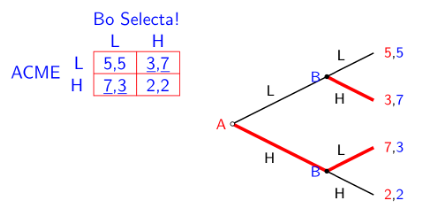
\includegraphics[width=9cm,height=4.5cm]{BF303-IMG/2.png}
        \end{center}

	\textbf{Figure 3: SHEP Progression Rate Comparison}

        \begin{center}
                
\includegraphics[width=9cm,height=4.5cm]{BF303-IMG/3.png}
        \end{center}

	\newpage

	\textbf{Model 1: Regressing Academic Potential w/ Intermediate Effect}\\

	\textbf{Causal Instrument}
	\begin{itemize}
	\setlength\itemsep{0cm}
		\item Area of Residence
		\item Type of School
		\item Resources Available
		\item Historic School Progression Rate
	\end{itemize}

	\textbf{Intermediary (Primary) Factors}
	\begin{itemize}
        \setlength\itemsep{0cm}            
                \item Family Income 
                \item Young Carers
                \item Family Problems/`Upbringing'
                \item Historic Family Trends
        \end{itemize}

	\textbf{Intermediary (Secondary) Factors}
	\begin{itemize}                               
        \setlength\itemsep{0cm}            
                \item Mental Health (Social)
                \item Behaviour (Social)
                \item Effort/Care for School (Social)
                \item Confidence (Social)
                \item Ability to Choose Subjects (K\&U)
                \item Lack of Belief in Ability to Attend University (K\&U)
                \item Understanding of University (K\&U)
                \item Implied Costs of University (K\&U)
		\item Burden of Student Debt (K\&U)
		\item Ability to Create Convincing Applicative Material (K\&U)
        \end{itemize}

	\textbf{Effect/Outcome}
        \begin{itemize}                               
        \setlength\itemsep{0cm}            
                \item Academic Response 
                \item Progression Rate
                \item Attainment of H.E. Qualifications
                \item Post-Graduate Earnings
        \end{itemize}

\newpage

	\renewcommand\refname{Bibliography}

        \begin{thebibliography}{9}

	\bibitem{a}
		Commission on Widening Access. (2016).
		\textsl{A Blueprint for Fairness: The Final Report of the Commission on Widening Access.}
		Commission on Widening Access.

	\bibitem{b}
		Hindricks, J., Myles, G. (2013).
		\textsl{Intermediate Public Economics.}
		MIT Press 2nd Edition.
	
	\bibitem{c}
		Hoxby, C. (1999).
		\textsl{The Productivity of Schools and Other Local Public Goods Producers.}
		Journal of Public Economics.

	\bibitem{d}
		Howieson, C., Lannelli, C. (2008).
		\textsl{The Effects of Low Attainment on Young People’s Outcomes at Age 22-23 in Scotland.}
		British Educational Research Journal.

	\bibitem{e}
		Koop, G. (2007).
		\textsl{Introduction to Econometrics.}
		John Wiley and Sons.

	\bibitem{f}
		MacLeod, W., Urquiola, M. (2009).
		\textsl{Anti-Lemons: School Reputation \& Educational Equality.}
		The National Bureau of Economic Research.

	\bibitem{g}
		Martin, J. (2010).
		\textsl{Stigma and Student Mental Health in Higher Education.}
		Journal of Higher Education Research \& Development

	\bibitem{h}
		Parsons, S., Bynner, J. (2007).
		\textsl{Illuminating Disadvantage: Profiling the Experiences of Adults with Every Level Literacy or Numeracy Over the Lifecourse.}
		National Research and Development Centre for Adult Literacy and Numeracy.

	\bibitem{i}
		Powis, D., James, D., Ferguson, E. (2007).
		\textsl{Demographic and Socio-Economic Associations with Academic Attainment (UCAS Tariff Scores) in Applicants to Medical School.}
		Medical Education.

	\bibitem{j}
		Scottish Funding Council (2014).
		\textsl{Schools for Higher Education Programme: 2014 Review of Activity: Final Report.}
		Edinburgh: Scottish Funding Council.

	\bibitem{k}
		Sosu, E., Ellis, S. (2014).
		\textsl{Closing the Attainment Gap in Scottish Education.}
		Joseph Rowntree Foundation.

	\bibitem{l}
		Sosu, E., Smith, L., McKendry, Santoro, N., Ellis, S. (2016). 
		\textsl{Widening Access to Higher Education for Students for, Economically Disadvantaged Backgrounds.}
		University of Strathclyde.

	\end{thebibliography}

\end{document}
